\chapter{Captura de telas da ferramenta implementada}
\label{apend-ferramenta}

Neste apêndice apresentamos em mais detalhes as partes da tela principal da ferramenta implementada.
Na Figura~\ref{fig-ferramenta-grafo} temos a tela principal da ferramenta,
para melhor descreve-la dividimos em cinco figuras, contendo as principais regiões.

\begin{figure}[h]
	\begin{center}
	    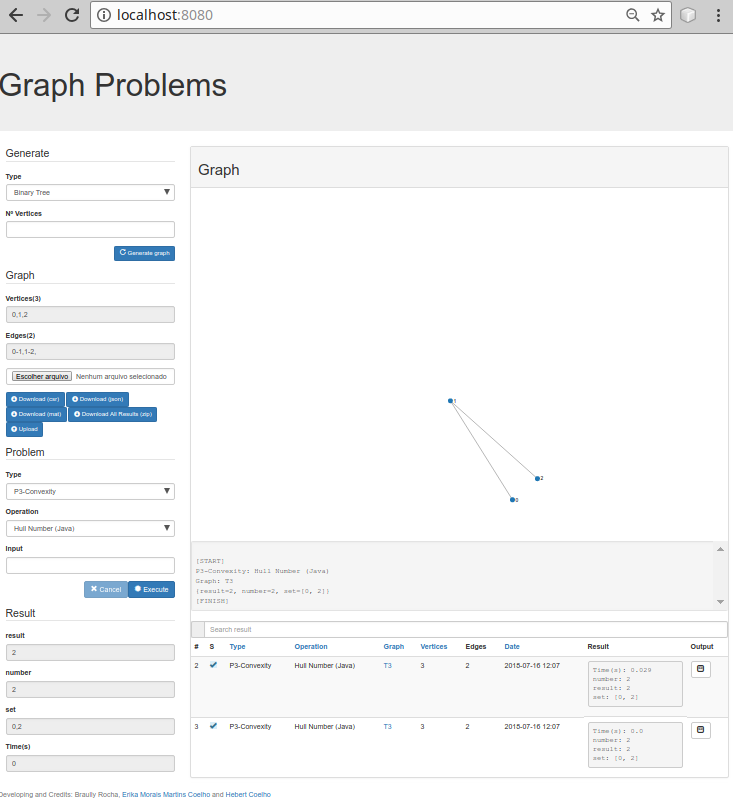
\includegraphics[width=0.8\textwidth]{./imagens/ferramenta-tela-principal.png}
	\end{center}
   	\caption{Ferramenta para Execução de Algoritmos}
    \label{fig-ferramenta-grafo}
\end{figure}

Na Figura~\ref{fig-ferramenta-grafo-tabela-resultados} 
temos a captura de tela da região de histórico de resultados executados.
No histórico é possível buscar resultados anteriores,
filtrar por algum termo, entre as informações apresentadas estão o problema, o grafo informado, a quantidade de vértices e arestas,
tempo de execução e o resultado do problema em si.

\begin{figure}[h]
	\begin{center}
	    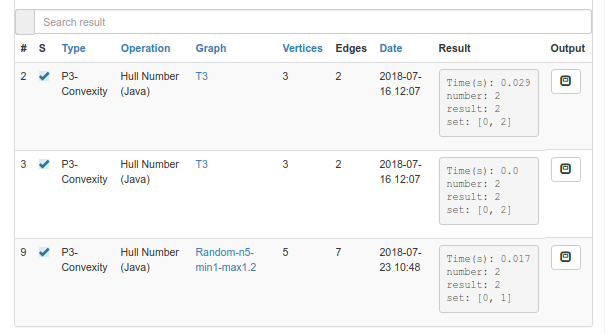
\includegraphics[width=0.8\textwidth]{./imagens/ferramenta-resultado.png}
	\end{center}
	\caption{Captura de Tela Histórico de Resultados}
    \label{fig-ferramenta-grafo-tabela-resultados}
\end{figure}

Na Figura~\ref{fig-ferramenta-grafo-console} temos a captura de tela da área que contem uma representação visual do grafo em uso e um console com as informações de qualquer operação em andamento.

\begin{figure}[H]
\begin{center}
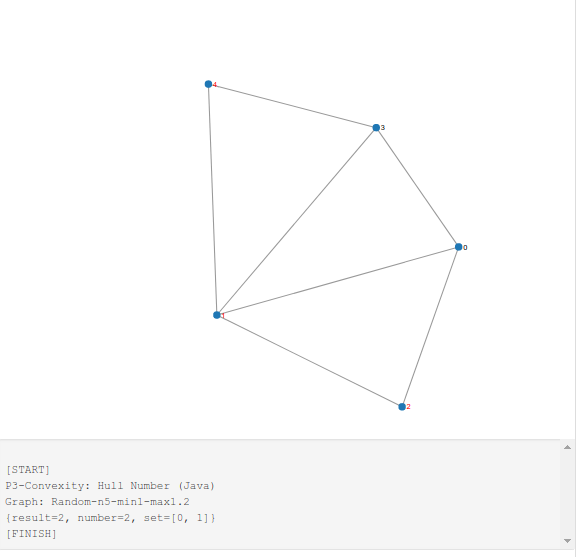
\includegraphics[width=0.5\textwidth]{./imagens/ferramenta-resultado-console.png}
\end{center}
\caption{Captura de Tela Imagem Grafo e Console de Execução}
\label{fig-ferramenta-grafo-console}
\end{figure}


Na Figura~\ref{fig-ferramenta-area-gerador} temos em maior detalhe a captura de tela da área de geração de grafo.

\begin{figure}[H]
	\begin{center}
	    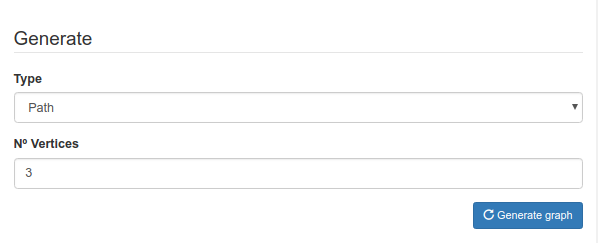
\includegraphics[width=0.5\textwidth]{./imagens/ferramenta-area-gerador.png}
	\end{center}
	\caption{Captura de Tela Geração de Grafo}
    \label{fig-ferramenta-area-gerador}
\end{figure}

Na Figura~\ref{fig-ferramenta-area-info-grafo} temos em maior detalhe a captura de tela da área de informações sobre o grafo.
Temos os vértices, lista de arestas, além dos botões que permitem baixar o grafo atual nos formatos \textit{csr}, \textit{json} e \textit{mat}.
Também está disponível um botão para baixar todos o histórico de resultados. 
Por fim também temos a opção de fazer o \textit{upload} de um arquivo contendo um grafo, nos mesmos formatos disponíveis para \textit{download}.

\begin{figure}[H]
\begin{center}
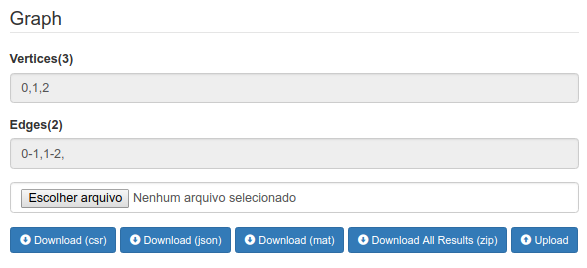
\includegraphics[width=0.5\textwidth]{./imagens/ferramenta-area-info-grafo.png}
\end{center}
\caption{Captura de Tela Geração de Grafo}
\label{fig-ferramenta-area-info-grafo}
\end{figure}


Na Figura~\ref{fig-ferramenta-area-problema} temos em maior detalhe 
a captura de tela da área de seleção do problema e o botão para executar a operação. Para problemas que exigem informações extras de entrada, 
existe uma caixa para digitação dessas informações.

\begin{figure}[H]
\begin{center}
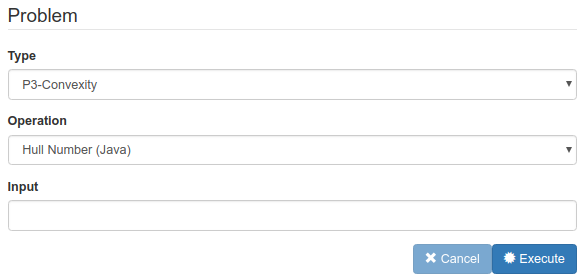
\includegraphics[width=0.5\textwidth]{./imagens/ferramenta-area-problema.png}
\end{center}
\caption{Captura de Tela Seleção de Problema}
\label{fig-ferramenta-area-problema}
\end{figure}



\chapter{Grafo Formato N,M,Índice}
\label{apend-nm-indice}
Neste trabalho grande parte das implementações exigiram combinações para soluções de problemas
e na geração de grafos. Por vezes se fez necessário uma forma simples de retomar a construção de um grafo,
com uma combinação do gerador de grafo completo e uso do índice lexicográfico para obter uma combinação,
elaboramos um gerador/formato de representação de um grafo partindo apenas de três números inteiros.

Considere o Algoritmo~\ref{alg:gera-kn} gerador de um grafo completo simples e não direcionado.
Dado que qualquer grafo de ordem $n$ é subgrafo de $K_n$ apenas removendo arestas. 
Se pudermos identificar na linha $9$ quais arestas não adicionar em $E$, 
o algoritmo pode ser utilizado para gerar qualquer grafo não direcionado. 


\begin{algorithm2e}[H]
    \SetAlFnt{\tiny}
    \SetAlCapFnt{\small}
    \SetAlCapNameFnt{\small}
    \SetAlgoLined
    \DontPrintSemicolon
    \LinesNumbered
    \SetAlgoLined
    \BlankLine
    \Entrada{$n$}
    \Saida{Grafo $G$ completo de ordem $n$}
    \BlankLine
    $V \gets \emptyset$ \\
    $E \gets \emptyset$ \\
    $rotulo \gets 0$ \\
    \Para{$i \gets 0$ \Ate $n-1$}{
    	$V\gets V \cup \{i\}$\\
    }        
    \Para{$i \gets 0$ \Ate $n-1$}{
    	\Para{$j \gets i+1$ \Ate $n-1$}{
    		$E \gets E \cup (i,j)$\\
            $rotulo \gets rotulo + 1$
    	}
    }
    \Retorna{$G(V,E)$} 
\caption{$GeraK_n(n)$}
\label{alg:gera-kn}
\end{algorithm2e} 

No Algoritmo~\ref{alg:gera-kn} sabemos que para uma entrada $n$, será gerado um grafo completo com $n$ vértices e consequentemente $m=\frac{n(n-1)}{2}$ arestas.  Podemos perceber que cada aresta poderia ser identificada de forma única por um rotulo gerado na linha 10. Se existe a priori um conjunto com todos os rótulos de arestas a serem gerados, 
poderia se adicionar em $E$ apenas as arestas desejadas, podendo assim gerar qualquer grafo $G$ de ordem $n$ desejado.


Seja $n$ o número de vértices, sabendo que $MaximoArestas(n)=\frac{n(n-1)}{2}$. Um conjunto contendo $k$ rótulos de arestas desejadas, nada mais é que uma combinação $C(MaximoArestas(n),k)$. Ao passo que qualquer combinação $C(a,b)$ pode ser obtida a partir de seu índice lexicográfico, desde que se conheça os valores de $a$, $b$. Podemos assim representar qualquer grafo de ordem $n$ com apenas 3 números: quantidade de vértices (n), arestas (m) e o índice lexicográfico (i).


Com pequenas alterações no algoritmo de geração de grafo completo podemos obter o Algoritmo~\ref{alg:gera-n}, que é capaz de gerar qualquer grafo a partir de três números inteiros. Vejamos um exemplo, seja $K_5$ o grafo retornado pelo Algoritmo~\ref{alg:gera-kn} para $n=5$, será gerado 10 arestas e com rótulos conforme Figura~\ref{fig-exemplos-algoritmos-geracao}. Os grafos $C_5$ e $W_5$ podem ser obtidos a partir de $K_5$ apenas removendo algumas arestas. Em $C_5$ as arestas desejadas são as de rótulo $R_{C_5}=\{1, 4, 5, 8, 10\}$. Ao passo que as arestas desejadas para se obter um $W_5$ são $R_{W_5}=\{1, 2, 3, 4, 5, 7, 8, 10\}$. A combinação de arestas para o dado $C_5$ é a de índice lexicográfico 99, portanto o mesmo grafo poderia ser gerado pelo Algoritmo~\ref{alg:gera-n} com os parâmetros $n=5$, $m=5$ e $i_{lex}=99$. Ao passo que para o $W_5$ o índice lexicográfico do conjunto de arestas é 32, podendo ser gerado pelo Algoritmo~\ref{alg:gera-n} com os parâmetros $n=5$, $m=8$ e $i_{lex}=32$.

Dado que um conjunto é uma combinação de dois números, esse conjunto pode ser facilmente convertido em um índice lexicográfico. O contrário também se confirma, dado o índice lexicográfico de uma combinação, podemos obter a combinação representada pelo índice. Assim temos uma forma diferente e interessante de se representar grafos.


\begin{algorithm2e}[H]
    \SetAlFnt{\tiny}
    \SetAlCapFnt{\small}
    \SetAlCapNameFnt{\small}
    \SetAlgoLined
    \DontPrintSemicolon
    \LinesNumbered
    \SetAlgoLined
    \BlankLine
    \Entrada{$n$, $m$ e $i_{lex}$}
    \Saida{Grafo $G$ completo de ordem $n$}
    \BlankLine
    $V \gets \emptyset$ \\
    $E \gets \emptyset$ \\
    $R \gets Combinacao(\frac{n(n-1)}{2},k,i_{lex})$\\
    $rotulo \gets 0$ \\
    \Para{$i \gets 0$ \Ate $n-1$}{
    	$V\gets V \cup \{i\}$\\
    }        
    \Para{$i \gets 0$ \Ate $n-1$}{
    	\Para{$j \gets i+1$ \Ate $n-1$}{
        	\Se{$rotulo\in R$} {
    			$E \gets E \cup (i,j)$\\
            }
            $rotulo \gets rotulo + 1$
    	}
    }
    \Retorna{$G(V,E)$} 
\caption{$GeraG(n,m,i_{lex})$}
\label{alg:gera-n}
\end{algorithm2e} 


\begin{figure}[h]
\centering
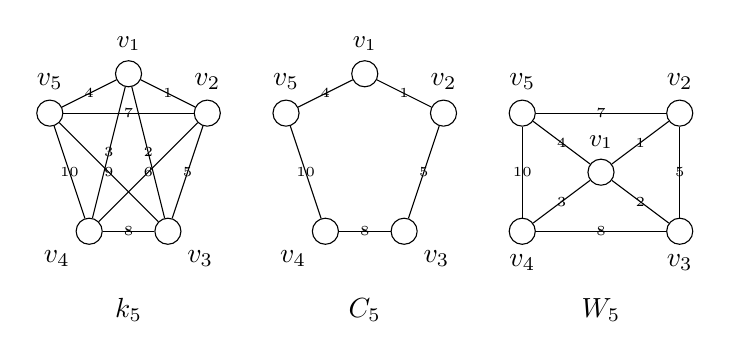
\begin{tikzpicture}
    \node[draw,circle,label={\small $v_1$}] (v1) at (-6,2) {};
\node[draw,circle,label=$v_2$] (v2) at (-5,1.5) {};
\node[draw,circle,label=below right:$v_3$] (v3) at (-5.5,0) {};
\node[draw,circle,label=below left:$v_4$] (v4) at (-6.5,0) {};
\node[draw,circle,label=$v_5$] (v5) at (-7,1.5) {};

\draw  (v1) -- node {\tiny $1$} (v2);
\draw  (v1) -- node {\tiny $2$}  (v3); 
\draw  (v1) -- node {\tiny $3$}  (v4);
\draw  (v1) -- node {\tiny $4$}  (v5);
\draw  (v2) -- node {\tiny $5$}  (v3);
\draw  (v2) -- node {\tiny $6$}  (v4);
\draw  (v2) -- node {\tiny $7$}  (v5);
\draw  (v3) -- node {\tiny $8$}  (v4);
\draw  (v3) -- node {\tiny $9$}  (v5);
\draw  (v4) -- node {\tiny ${10}$}  (v5);
\node at (-6,-1) {$k_5$};


\node[draw,circle,label={\small $v_1$}] (v21) at (-3,2) {};
\node[draw,circle,label=$v_2$] (v22) at (-2,1.5) {};
\node[draw,circle,label=below right:$v_3$] (v23) at (-2.5,0) {};
\node[draw,circle,label=below left:$v_4$] (v24) at (-3.5,0) {};
\node[draw,circle,label=$v_5$] (v25) at (-4,1.5) {};

\draw  (v21) -- node {\tiny $1$} (v22);
\draw  (v21) -- node {\tiny $4$}  (v25);
\draw  (v22) -- node {\tiny $5$}  (v23);
\draw  (v23) -- node {\tiny $8$}  (v24);
\draw  (v24) -- node {\tiny ${10}$}  (v25);
\node at (-3,-1) {$C_5$};

\node[draw,circle,label={\small $v_1$}] (v31) at (0,0.75) {};
\node[draw,circle,label=$v_2$] (v32) at (1,1.5) {};
\node[draw,circle,label=below:$v_3$] (v33) at (1,0) {};
\node[draw,circle,label=below:$v_4$] (v34) at (-1,0) {};
\node[draw,circle,label=$v_5$] (v35) at (-1,1.5) {};

\draw  (v31) -- node {\tiny $1$} (v32);
\draw  (v31) -- node {\tiny $2$}  (v33); 
\draw  (v31) -- node {\tiny $3$}  (v34);
\draw  (v31) -- node {\tiny $4$}  (v35);
\draw  (v32) -- node {\tiny $5$}  (v33);

\draw  (v32) -- node {\tiny $7$}  (v35);
\draw  (v33) -- node {\tiny $8$}  (v34);
\draw  (v34) -- node {\tiny ${10}$}  (v35);
\node at (0,-1) {$W_5$};
\end{tikzpicture}
\caption{Grafos gerados pelos Algoritmos~\ref{alg:gera-kn} e~\ref{alg:gera-n}} 
\label{fig-exemplos-algoritmos-geracao}
\end{figure}



% \chapter{Conjecturas e Ensaios de Demonstração}
% Neste apêndice apresentamos algumas ideias exploradas em cima das conjecturas investigadas, apesar de não concluídos os estudos, deixamos aqui para registro e futuros trabalhos.

% % \begin{conjecture}
% %     Seja $G$ um grafo com diâmetro 2, então $c(G) \le 4$.
% %     \label{conjecture-g-c4}
% % \end{conjecture}

% % \begin{conjecture}
% %     Seja $G$ um grafo e $d$ seu diâmetro, então $c(G) \le d^2$.
% %     \label{conjecture-d2-c4}
% % \end{conjecture}

% % \begin{conjecture}
% %     Seja $G$ um grafo com diâmetro 2, sem vértice de corte então $h(G) \le 4$.
% %     \label{conjecture-d2-4}
% % \end{conjecture}

% A Conjectura~\ref{conjecture-d2-4} foi a mais investigada no decorrer do trabalho, permanecendo em aberta  e exigem mais investigação, dois possíveis caminhos mais promissores para a demonstração estão apresentados aqui. 


% No primeiro caminho usando a propriedade de dominação total da vizinhança de qualquer vértice de um grafo de diâmetro 2, juntamente com o principio da casa do pombos, segue uma possível demonstração.    
%     Seja $v_1$ um vértice de $G$, tal que $d(v_1)=\Delta(G)$. Faça $S_1=\{v_1\}$, $H(S_1)$ e $R_1=V(G) \setminus N(H(S_1))$, se $R_1$ é vazio então $S_1$ é dominante, caso contrário sabemos que $R_1 < n-\Delta$. Se $S_1$ não é envoltório então pelo principio da casa dos pombos existe um vértice $v_2$, tal que $d(v_2) \ge \lceil \frac{n-\Delta}{\Delta} \rceil$. Faça $S_2=\{v_1,v_2\}$, $H(S_2)$ e $R_2=V(G) \setminus N(H(S_2))$, se $R_2$ é dominante então $|S_2|+1$ é envoltório, sabemos então que $R_2 < n - \Delta - \lceil \frac{n-\Delta}{\Delta} \rceil$. Se $S_2$ não é envoltório então pelo principio da casa dos pombos existe um vértice $v_3$, tal que $d(v_3) \ge \lceil \frac{n-\Delta - \lceil \frac{n-\Delta}{\Delta} \rceil }{\Delta-1} \rceil$ e assim sucessivamente, podemos estabelecer uma relação de recorrência para o conjunto $R_i=n-T(i-1)$ tal que: 
    
%      $$
%       T(0) = \Delta 
%       T(i) =  \Big\lceil \frac{\Delta - i - 1}{\Delta-i} \times (T(i-1)+n) \Big\rceil 
%     $$
%     Em um grafo cujo $\Delta$ seja elevado, $R_i$ será vazio em poucas iterações, tal como $\Delta=n-2$ em que o $R_i$ será zero na segunda iteração. Porém quando $\Delta$ assume o minimo valor possível, mais iterações são necessárias. Pelas propriedades de um grafo diâmetro 2 minimal, o menor valor possível para $\Delta$ é $\sqrt[]{n-1}$ substituindo esse valor na equação de recorrência, e resolvendo a equação, é possível saber para qualquer grafo de ordem $n$ em qual iteração $i$ o valor de $R_i \le 0$. Se encerrar em uma constante, temos assim o primeiro possível caminho de demonstração da conjectura.
    
% Em uma possível demonstração mais direta, baseada apenas nas propriedades de que para qualquer dois vértices em um grafo de diâmetro 2, ou são vizinhos ou tem um vizinho em comum. Segue um outro possível caminho de demonstração.
% 	Se $G$ é um grafo de diâmetro 2, necessariamente existem pelo menos dois vértices não adjacentes. Caso contrário, $G$ seria um grafo completo e um grafo completo possui diâmetro é 1.
    
%     Seja $v_1,v_2\in V(G)$ dois vértices distintos e não adjacentes. Como $G$ é um grafo de diâmetro 2 então existe um vértice $z \in V(G)$ tal que $v_1z, v_2z \in E(G)$. Considere $S_1=\{v_1, v_2\}$. Note que $z \in H(S_1)$. Agora, vamos separar os vértices de $G$ em dois conjuntos, $H(S_1)$ e $V(G) \setminus H(S_1)$. 
    
%     Como não existe vértice de corte em G, $v_1$ e $v_2$ possuem outros vizinhos, não necessariamente em comum, diferentes de $z$. Se $N(u) \subseteq H(S_1)$, $u \in H(S_1)$, então pela Proposição \ref{pro-diam-2-itemb} $H(S_1)$ é um conjunto dominante. Logo pelo Lema \ref{hs-dominante-envoltorio} $S_1 \cup \{v\}$ é um conjunto envoltório, para $v \in V(G) \setminus H(S_1)$. Portanto $h(G)\le 3$.
    
%     Agora, considere que todo vértice de $H(S_1)$ possua pelo menos um vizinho em $V(G) \setminus H(\{S_1\})$. Note que não existe $v \in V(G) \setminus H(\{S_1\})$ que pertença a vizinhança de quaisquer dois vértices de $H(S_1)$. Caso contrário, $v$ pertenceria a $H(S_1)$. 
    
%     Considere $v_3 \in V(G) \setminus H(\{S_1\})$ tal que $v_2v_3 \in E(G)$. Faça $S_2=\{v_1, v_2, v_3\}$. Observe que $v_1v_3 \notin E(G)$, então existe um vértice $u \in V(G) \setminus H(\{S_1\})$ tal que $uv_1, uv_3 \in E(G)$. Dessa forma existe um ciclo de tamanho cinco, $C=v_1, z, v_2, v_3, u$. Caso $V(G)\setminus H(S_2)=\emptyset$ então $h(G)\le 3$.
    
% %    Caso $V(G) \setminus H(S_2) \ne \emptyset$. Se $V(G) \setminus N(H(S_2)) = \emptyset$ então pelo Lema~\ref{hs-dominante-envoltorio} $G$ tem um conjunto envoltório $S_2\cup \{v\}$, logo $h(G)\le 4$. Caso $V(G) \setminus N(H(S_2)) \ne \emptyset$ e $\exists v \in V(G) \H(S_2) | N(v) \subset N(H(S))$ então pelo Lema~\ref{hs-dominante-envoltorio} $G$ tem um conjunto envoltório $S_2\cup \{v\}$, logo $h(G)\le 4$.

%      Caso $V(G) \setminus H(S_2) \ne \emptyset$. Se $V(G) \setminus N(H(S_2)) = \emptyset$ então pelo Lema~\ref{hs-dominante-envoltorio} $G$ tem um conjunto envoltório $S_2\cup \{v\}$, logo $h(G)\le 4$.  Caso $V(G) \setminus N(H(S_2)) \ne \emptyset$ e $\exists v \in V(G) \setminus H(S_2) | N(v) \subset N(H(S))$ então pelo Lema~\ref{hs-dominante-envoltorio} $G$ tem um conjunto envoltório $S_2\cup \{v\}$, logo $h(G) \le 4$.
    
%     Permanecendo em aberto o caso final em que $\forall v \in V(G)\setminus N(H(S_2))$ v é adjacente a outro vértice em $V(G) \setminus N(H(S_2))$. Conjuntos $H=H(S_2)$, $N=N(H(S_2)) \setminus H(S_2)$ e $R=V(G) \setminus N(H(S_2))$. Para este ultimo caso, segue as observações levantadas:
%      \begin{itemize}
%      \item{Observação-1: Todo vértice $v$ em $R$ possui $|H(S)|$ de seus vizinhos em $N$. Esse vértices de $v$ em $N$ possuem grau minimo $|H(S)|$ }
%      \item{Observação-2: Os vértices adjacente de $v$ que também estejam em $R$ possuem grau minimo 5.}
%      \item{Observação-4: Para todo vértice $v$ em $R$: Pela casa dos pombos $N[v]$ domina $N-N[v]$ e existe um vértice de grau $\frac{|N|-|H(S)|}{d(v)}$ .}
%      \item{Observação-5: Os vértices adjacente de $v$ que também estejam em $R$ precisam dominar $N(C_5)$.}
%      \end{itemize}
     
% %Todo vértice $v$ em $R$ pode ter no máximo $x$ vizinhos em $R$. Sendo $x=\lceil\frac{|N|-|H(S)}{\Delta-1}\rceil$. E o grau minimo de $v$ é $d(v) \ge |H(S)|+\lceil\frac{|N|-|H(S)}{\Delta-1}\rceil$

% %Sabemos que $d(v)=\Delta$. Desenvolvendo a expressão

% %$d(v) \ge |H(S)|+\lceil\frac{|N|-|H(S)}{\Delta-1}\rceil \le \Delta$

% %$d(v) \ge \lceil\frac{|N|-(\Delta-2)|H(S)}{\Delta-1}\rceil \le \Delta$

% %$\lceil\frac{|N|-(\Delta-2)|H(S)}{\Delta-1}\rceil \le \Delta$



